\chapter{Design Requirements \& Architecture}

This chapter outlines the design requirements and architecture of the \texttt{tinyC} compiler frontend. First, it defines the functional and non-functional requirements that guide the design decisions. Then, it analyses the \texttt{tinyC} grammar to understand its characteristics and challenges. Finally, it describes the system architecture, including the AST design, API specifications, and test suite architecture.

\section{Functional Requirements}

The primary purpose of the \texttt{tinyC} compiler frontend is to provide students with a reliable tool for parsing \texttt{tinyC} source code, allowing them to focus on compiler middle-end and back-end development in the language of their choice. The functional requirements define the essential capabilities the system must provide to fulfill this purpose.

\subsection{Core Parsing Functionality}
At its heart, the frontend must perform accurate lexical analysis by tokenizing \texttt{tinyC} source code according to the language specification. This process involves correctly identifying all token types—keywords, identifiers, literals, operators, and punctuation—while properly managing whitespace and comments. The frontend then conducts syntax analysis, parsing the token stream according to the \texttt{tinyC} grammar rules to verify syntactic correctness.

Upon successful parsing, the system constructs a well-structured abstract syntax tree (AST) that accurately represents the parsed program's hierarchical structure. This AST serves as the primary interface between the frontend and any student-implemented backend. To facilitate error reporting and debugging throughout the compilation process, each node in the AST includes precise source location information, including filename, line number, and column number.


\subsection{Error Handling}
Effective error handling constitutes a critical aspect of the frontend's functionality. The system detects and reports lexical errors (such as invalid characters or malformed tokens), and syntactic errors (such as grammar violations). More importantly than merely detecting these errors, the frontend provides clear, informative error messages that include relevant source location information. These messages guide students toward understanding and resolving issues in their code, enhancing the educational value of the tool.


\subsection{Interface Options}
The frontend offers two complementary interface options to accommodate different student preferences and project requirements. First, a C++ library interface provides direct access to AST classes and parsing functionality. This option is ideal for students who prefer working in C++ and wish to tightly integrate the frontend with their backend implementation.

Second, a command-line interface provides a standalone executable that accepts \texttt{tinyC} source files and outputs the AST in JSON format. This interface option enables students to work in any programming language of their choice, as they can parse the standardized JSON output using libraries available in virtually any language.

The JSON output follows a well-defined schema that includes all necessary information from the AST, including node types, hierarchical relationships, and source locations. This schema ensures consistency and interoperability regardless of which backend implementation approach a student chooses.


\section{Non-functional Requirements}

While functional requirements define what the system must do, non-functional requirements define the qualities that determine how the system should behave. These requirements are crucial for ensuring the frontend's suitability for its educational context and for providing a positive experience for students using it in their coursework.


\subsection{Performance}
The frontend must perform efficiently enough to handle typical \texttt{tinyC} programs without introducing frustrating delays in the development workflow. Parsing time should scale proportionally with input size, maintaining reasonable performance even for larger programs. 

Memory usage should remain modest, avoiding unnecessary duplication of data and implementing appropriate data structures for the AST nodes. Since the frontend will be used primarily in an educational setting, absolute performance optimization is less critical than clarity and correctness, but the implementation should still follow reasonable efficiency principles.


\subsection{Usability}
For the frontend to serve its educational purpose effectively, it must be straightforward to integrate into student projects. This requires minimal external dependencies, clear documentation, and intuitive interfaces. The API, JSON format, and usage examples need documentation that students can reference without extensive prior knowledge of compiler construction. Installation and setup should be simple, with clear instructions for different operating systems.

Platform independence is essential, as students in the course may use various development environments across Windows, macOS, and Linux. The frontend should function consistently across these platforms, avoiding system-specific features that might create barriers for some students. For the command-line interface, the output format should be consistent regardless of the operating system, ensuring that student backends can rely on a standardized input format.


\subsection{Maintainability}
The implementation must be clean, well-structured, and follow modern C++ best practices to facilitate future maintenance and extension. A modular design separates concerns like lexical analysis, syntax analysis, and AST construction, making each component easier to understand and modify independently. The JSON output format and AST structure are designed with extensibility in mind, allowing for potential future extensions to the \texttt{tinyC} language without requiring a complete redesign.

The codebase requires unit tests for both the lexer and parser components to verify their correctness independently. These unit tests should cover a wide range of input cases, including edge cases and error conditions, ensuring that each component behaves as expected in isolation before being integrated. This approach facilitates a more maintainable codebase where changes to one component do not inadvertently affect others.

The codebase should be maintained in a version control system with a clear commit history, enabling instructors to track changes and understand the evolution of the implementation. This approach also supports potential contributions from teaching assistants or even students in future course iterations.


\subsection{Educational Value}
Given its pedagogical context, the frontend must serve not only as a functional tool but also as a learning resource. The code should be readable and instructive, serving as a good example for students learning about compiler construction. Implementation choices should balance theoretical correctness with practical considerations, demonstrating sound software engineering principles alongside compiler theory.

Beyond unit tests, the system requires a language test suite that verifies the frontend's behavior against a collection of \texttt{tinyC} programs. This test suite serves multiple purposes: it validates the correctness of the provided implementation, gives students a tool to verify their own implementations, and demonstrates the expected behavior of the language across various scenarios. The test suite should include specially formatted \texttt{tinyC} source files with metadata specifying expected outcomes, enabling automated validation of parser behavior.

The test suite should support incremental development, allowing students to focus on specific language features one at a time. It should provide clear feedback about why tests fail, helping students identify and fix issues in their implementations. Additionally, the test suite should cover both successful parsing cases and error conditions, ensuring that parsers correctly handle invalid input.

\section{\texttt{tinyC} Grammar Analysis}

The \texttt{tinyC} language is a simplified subset of C designed for educational purposes. Understanding its grammar characteristics and implementation challenges is essential for designing an effective parser that serves the course's pedagogical goals.

The \texttt{tinyC} language encompasses a carefully selected subset of C language features, providing enough complexity to be educational while remaining manageable for a course project. It supports basic types including integer, double, character, and void types, along with variables, arrays, and pointers. Function declarations and definitions follow C-like syntax, and the language includes standard control structures—if-else conditionals, while and do-while loops, for loops, and switch-case statements. Expression syntax maintains C-like operator precedence, and the language supports struct definitions for creating custom data types.

From a formal language perspective, the \texttt{tinyC} grammar can be generally classified as LL(1), making it suitable for implementation using predictive recursive descent parsing techniques. This classification is particularly advantageous in an educational context, as recursive descent parsers closely mirror the grammar's structure, making the relationship between theory and implementation more transparent to students. To verify the LL(1) properties of the grammar and to assist with implementation, I used a parsing table generator tool developed by Ing. Tomáš Pecka (available at \url{pages.fit.cvut.cz/peckato1/parsingtbl}). This tool proved invaluable for identifying and resolving grammar conflicts, as well as for generating templates for recursive descent parsing functions.

Several aspects of the \texttt{tinyC} grammar presented challenges for implementing a pure LL(1) parser. Expression parsing required careful factoring to eliminate left recursion while preserving operator precedence. Type declarations, especially pointer types and function pointers, needed special handling to account for their complex syntax. Statements with optional components like the for-loop's initialization, condition, and update expressions required nullable productions and appropriate lookahead testing. Additionally, the original grammar contained instances of left recursion and common prefixes that needed systematic elimination through standard grammar transformations to ensure LL(1) compatibility.

The final grammar used for implementation is provided in Appendix~\ref{app:grammar}. It represents a factored form of the \texttt{tinyC} grammar that is suitable for LL(1) parsing while remaining faithful to the language specification. While the transformations introduce some additional non-terminals and productions compared to the original grammar, they preserve the language's semantics and ensure efficient, predictable parsing behavior.

\section{System Architecture}

The \texttt{tinyC} compiler frontend is designed with a modular architecture that separates concerns and facilitates both maintenance and extension. Figure~\ref{fig:architecture} illustrates the high-level architecture of the system.

\begin{figure}[ht]
    \centering
    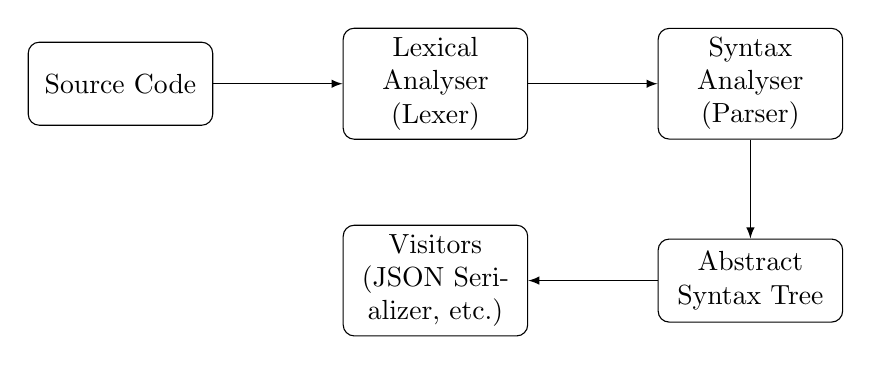
\begin{tikzpicture}[node distance=2cm, auto]
      % Define block styles
      \tikzstyle{block} = [rectangle, draw, text width=6em, text centered, rounded corners, minimum height=3em]
      \tikzstyle{line} = [draw, -latex]
      
      % Place blocks
      \node [block] (source) {Source Code};
      \node [block, right of=source, node distance=4cm] (lexer) {Lexical Analyser (Lexer)};
      \node [block, right of=lexer, node distance=4cm] (parser) {Syntax Analyser (Parser)};
      \node [block, below of=parser, node distance=2.5cm] (ast) {Abstract Syntax Tree};
      \node [block, left of=ast, node distance=4cm] (visitor) {Visitors (JSON Serializer, etc.)};
      
      % Draw lines
      \path [line] (source) -- (lexer);
      \path [line] (lexer) -- (parser);
      \path [line] (parser) -- (ast);
      \path [line] (ast) -- (visitor);
    \end{tikzpicture}
    \caption{High-level architecture of the \texttt{tinyC} compiler frontend}
    \label{fig:architecture}
\end{figure}

\pagebreak
The architecture consists of the following main components:

\begin{enumerate}
    \item \textbf{Lexical Analyser (Lexer)}: The lexer reads the source code character by character and groups them into tokens according to the lexical rules of \texttt{tinyC}. It handles whitespace, comments, and reports lexical errors.

    \item \textbf{Syntax Analyser (Parser)}: The parser takes the token stream produced by the lexer and verifies that it conforms to the \texttt{tinyC} grammar. It constructs an abstract syntax tree and reports syntax errors.

    \item \textbf{Abstract Syntax Tree (AST)}: The AST represents the hierarchical structure of the parsed program. Each node in the tree corresponds to a language construct in the source code.
    
    \item \textbf{Visitors}: The visitor pattern is implemented to traverse the AST for various operations. The most important visitor is the JSON serializer, which converts the AST to a standardized JSON representation. Other potential visitors could include a pretty-printer, static analyzer, or code generator.
\end{enumerate}

The core implementation is structured as a library (lib\texttt{tinyC}) that can be used directly in C++ projects. A separate command-line interface (\texttt{tinyC}-compiler) is built on top of this library, providing the standalone executable functionality.

\section{AST Design}

The AST design follows object-oriented principles to create a clear, maintainable, and extensible representation of \texttt{tinyC} programs. The design prioritizes simplicity, allowing students to easily work with the AST representation regardless of their implementation language.

\subsection{Node Structure}

The AST consists of various node types that represent different language constructs in \texttt{tinyC}. Rather than implementing a monolithic node class with numerous type-specific fields, the design employs a class hierarchy with a common base class (\texttt{ASTNode}) and specialized derived classes for different language elements. This approach follows the Single Responsibility Principle, with each class representing exactly one language construct.

Key node categories include declaration nodes for variables, functions, and structs; type nodes representing primitive types, named types, and pointer types; expression nodes for literals, identifiers, and operations; and statement nodes for blocks, conditionals, loops, and other control structures. Each node contains specific fields relevant to its language construct and provides access methods that expose these fields while maintaining appropriate encapsulation.

The base \texttt{ASTNode} class establishes common functionality across all nodes, including source location tracking for error reporting. Each derived class extends this base with construct-specific fields and behavior. This inheritance hierarchy allows for both static type safety through C++'s type system and runtime type identification through virtual functions and the visitor pattern.

\subsection{Memory Management}

The AST uses \texttt{std::unique\_ptr} for managing node ownership, a choice that naturally aligns with the hierarchical structure of abstract syntax trees. In an AST, each node has exactly one parent (except the root), creating a clear ownership hierarchy that unique pointers enforce at compile time. This approach offers several advantages over alternatives like \texttt{std::shared\_ptr}.

Unique pointers eliminate the reference counting overhead of shared pointers—an unnecessary cost for tree structures with clear parent-child relationships. They also prevent circular reference problems that could arise with shared pointers if the AST implementation needed cross-references between nodes. When using unique pointers, such relationships must be implemented as non-owning raw pointers, making ownership direction explicit and preventing accidental memory leaks.

From a design perspective, unique pointers make ownership transfer explicit through \texttt{std::move}, clearly indicating when a node becomes part of the parent structure. This explicitness improves code readability—particularly valuable in an educational context—while ensuring deterministic destruction that follows the tree hierarchy when nodes are deleted. This approach balances memory safety with performance considerations while maintaining a clear, understandable implementation.


\subsection{Visitor Pattern Implementation}

The visitor pattern provides a mechanism for performing operations on the AST without modifying the node classes, adhering to the Open-Closed Principle. This design pattern is particularly valuable in compiler construction, where different passes (e.g., semantic analysis, optimization, code generation) need to traverse the same AST structure while performing different operations.

The base \texttt{NodeVisitor} interface declares virtual \texttt{visit} methods for each concrete node type, as shown in Listing~\ref{code:node-visitor-interface}:

\begin{listing}[!h]
\begin{minted}{cpp}
class NodeVisitor {
public:
    virtual ~NodeVisitor() = default;
    
    // Visit methods for declaration nodes
    virtual void visit(const VariableNode& node) = 0;
    virtual void visit(const FunctionDeclarationNode& node) = 0;
    // ... other declarations
    
    // Visit methods for type nodes
    virtual void visit(const PrimitiveTypeNode& node) = 0;
    // ... other types
    
    // Visit methods for expression nodes
    virtual void visit(const LiteralNode& node) = 0;
    // ... other expressions
    
    // Visit methods for statement nodes
    virtual void visit(const BlockStatementNode& node) = 0;
    // ... other statements
};
\end{minted}
\caption{NodeVisitor interface declaration}
\label{code:node-visitor-interface}
\end{listing}

Each AST node implements an \texttt{accept} method that invokes the appropriate \texttt{visit} method on the visitor, as demonstrated in Listing~\ref{code:block-stmt-node-accept}:

\begin{listing}[ht!]
\begin{minted}{cpp}
void BlockStatementNode::accept(NodeVisitor& visitor) const {
    visitor.visit(*this);
}
\end{minted}
\caption{BlockStatementNode's accept method}
\label{code:block-stmt-node-accept}
\end{listing}

This design allows for adding new operations on the AST without modifying the node classes, adhering to the Open-Closed Principle as discussed in the visitor pattern implementation.



\subsection{Source Location Tracking}

Each AST node includes source location information to facilitate error reporting and debugging, as shown in Listing~\ref{code:ast-node-base-class}:

\begin{listing}[h!]
\begin{minted}{cpp}
class ASTNode {
public:
    explicit ASTNode(lexer::SourceLocation location);
    virtual ~ASTNode() = default;
    
    [[nodiscard]] lexer::SourceLocation getLocation() const;
    
    virtual void accept(NodeVisitor& visitor) const = 0;

private:
    const lexer::SourceLocation location;
};
\end{minted}
\caption{ASTNode base class declaration}
\label{code:ast-node-base-class}
\end{listing}

The \texttt{SourceLocation} struct contains the filename, line number (1-based), and column number (1-based). This information originates in the lexer, which tracks position as it tokenizes the source code. The parser then passes this location information to created AST nodes, ensuring that every node can be traced back to its origin in the source code.

This location tracking is particularly valuable for error reporting during later compilation phases. When a semantic error is detected (e.g., type mismatch or undeclared variable), the compiler can provide precise information about where the error occurred, greatly assisting students in debugging their \texttt{tinyC} programs.


\section{API Design}

The \texttt{tinyC} compiler frontend provides two main interfaces: a C++ library API for direct integration into student projects and a command-line interface for language-agnostic usage. This dual approach maximizes flexibility, accommodating students with varying programming language preferences and experience levels.


\subsection{Library API}

The library API allows direct integration of the \texttt{tinyC} frontend into C++ projects. This approach is ideal for students who prefer working in C++ and want tight integration between the frontend and their backend implementation. The API is designed with simplicity and clarity in mind, providing intuitive access to the frontend's core functionality.
The main entry point for lexical analysis is the \texttt{Lexer} class, shown in Listing~\ref{code:lexer-interface}:
\begin{listing}[ht!]
    \begin{minted}{cpp}
    namespace tinyC::lexer {
        class Lexer {
        public:
            explicit Lexer(std::string source, 
                           std::string filename = "<input>");
            TokenPtr nextToken();
            std::vector<TokenPtr> tokenize();
        };
    }
    \end{minted}
    \caption{Lexer class interface}
    \label{code:lexer-interface}
\end{listing}

The \texttt{Lexer} constructor accepts the source code as a string, along with an optional filename for error reporting. The \texttt{nextToken} method returns the next token in the input stream, while the \texttt{tokenize} method processes the entire input and returns a vector of all tokens. This design allows for both incremental token-by-token processing and batch processing of the entire input.

For syntax analysis, the \texttt{Parser} class provides the entry point, as shown in Listing~\ref{code:parser-interface}:

\begin{listing}[ht!]
\begin{minted}{cpp}
namespace tinyC::parser {
    class Parser {
    public:
        explicit Parser(lexer::Lexer& lexer);
        ast::ASTNodePtr parseProgram();
    };
}
\end{minted}
\caption{Parser class interface}
\label{code:parser-interface}
\end{listing}

The \texttt{Parser} constructor takes a reference to a \texttt{Lexer} instance, establishing the token source. The \texttt{parseProgram} method initiates parsing of the entire program, returning the root node of the resulting AST. This approach decouples the lexer and parser, allowing for separate testing and potential reuse of the lexer with different parsers.

For AST traversal and processing, the library provides visitor classes that implement the \texttt{NodeVisitor} interface, as shown in Listing~\ref{code:visitor-classes}:

\begin{listing}[ht!]
\begin{minted}{cpp}
namespace tinyC::ast {
    class DumpVisitor : public NodeVisitor {
    public:
        explicit DumpVisitor(std::ostream& os);
        // Visit methods for all node types
    };
    
    class JSONVisitor : public NodeVisitor {
    public:
        explicit JSONVisitor(bool prettyPrint = true);
        std::string getJSON() const;
        // Visit methods for all node types
    };
}
\end{minted}
\caption{Visitor classes for AST traversal}
\label{code:visitor-classes}
\end{listing}

The \texttt{DumpVisitor} outputs a human-readable representation of the AST to the specified output stream, useful for debugging and understanding the parsed structure. The \texttt{JSONVisitor} converts the AST to its JSON representation, with control over formatting through the \texttt{prettyPrint} option. The resulting JSON can be retrieved as a string using the \texttt{getJSON} method.

This API design prioritizes flexibility and ease of use. Students can work directly with the AST classes, implement their own visitors for custom operations, and control the parsing process step by step. The clear separation of concerns between lexical analysis, syntax analysis, and AST processing provides a solid foundation for understanding compiler structure.


\subsection{Command-Line Interface}

The command-line interface provides a standalone executable for parsing \texttt{tinyC} source files and outputting the AST as JSON. The main functionalities include:

\begin{enumerate}
    \item \textbf{Lexical Analysis Mode}: The command \texttt{tinyC-compiler --lex file.tc} tokenizes the input file and outputs the tokens. This mode is useful for debugging lexical issues and understanding how the source code is tokenized.

    \item \textbf{Parsing Mode}: The command \texttt{tinyC-compiler --parse file.tc} parses the input file and outputs the AST as JSON. This is the primary mode for students implementing their own backends, as it provides the complete AST structure in a standardized format.

    \item \textbf{Interactive Mode}: Running \texttt{tinyC-compiler} without arguments launches an interactive shell where students can enter \texttt{tinyC} code and immediately see the resulting tokens or AST. This mode is particularly useful for learning and experimentation.
\end{enumerate}

The command-line interface is designed to be simple and intuitive, with clear error messages and help text, making it accessible to students with varying levels of experience.

\subsection{JSON Output Format}
The JSON output format provides a standardized representation of the AST that can be consumed by any programming language. This format is the key to enabling language-agnostic backend implementation, as it decouples the frontend from any specific programming language or framework.

The JSON representation follows a well-defined schema with these key characteristics:

\begin{enumerate}
    \item \textbf{Node Type Identification}: Each node includes a \texttt{nodeType} field that identifies its type, allowing backends to process nodes according to their specific language construct.
    \item \textbf{Hierarchical Structure}: The JSON structure mirrors the hierarchical structure of the AST, with parent nodes containing their children as nested objects or arrays.
    \item \textbf{Source Locations}: Each node includes location information with filename, line, and column, enabling precise error reporting in later compilation phases.
    \item \textbf{Type-Specific Fields}: Each node type includes fields specific to that language construct, providing all necessary information for backend processing.
\end{enumerate}

An example JSON output for a simple variable declaration illustrating these characteristics is shown in Listing~\ref{code:json-example}.

\begin{listing}[h!]
\begin{minted}{json}
{
  "nodeType": "Program",
  "declarations": [
    {
      "nodeType": "VariableDeclaration",
      "identifier": "x",
      "type": {
        "nodeType": "PrimitiveType",
        "kind": "int",
        "location": {
          "filename": "example.tc",
          "line": 1,
          "column": 1
        }
      },
      "initializer": {
        "nodeType": "Literal",
        "kind": "integer",
        "value": "42",
        "location": {
          "filename": "example.tc",
          "line": 1,
          "column": 7
        }
      },
      "location": {
        "filename": "example.tc",
        "line": 1,
        "column": 5
      }
    }
  ],
  "location": {
    "filename": "example.tc",
    "line": 1,
    "column": 1
  }
}
\end{minted}
\caption{Example JSON output for a variable declaration: \texttt{int x = 42;}}
\label{code:json-example}
\end{listing}

This example demonstrates how the JSON format captures the hierarchical structure of the AST, with the program containing a variable declaration that includes a type and an initializer expression. Each node includes its type and location information, providing a complete representation of the parsed program.



\pagebreak







\section{Test Suite Architecture}
The test suite for the \texttt{tinyC} compiler frontend is a comprehensive framework designed to validate the correctness of both the provided implementation and student-created alternatives. It offers systematic verification of lexical analysis, parsing functionality, and error handling capabilities.

\subsection{Test File Structure and Format}
The test files follow a metadata-driven format that allows precise specification of expected outcomes. Each test file contains:

\begin{listing}[h!]
\begin{minted}{text}
// tinyC TEST
// INFO: description of the test's purpose
// RUN: test type specification (parser, exec)
// EXPECT: expected outcome (SUCCESS, PARSER_ERROR, or LEXER_ERROR)
// RESULT: expected JSON output (for SUCCESS tests only)

// Actual TinyC code follows...
\end{minted}
\caption{Example test file structure showing the required metadata header}
\label{code:test-file-structure}
\end{listing}

This approach separates test expectations from the code being tested, making it easier to understand the purpose of each test and to verify correct functionality. The addition of the \texttt{RUN} directive enables the test framework to support different testing modes, particularly distinguishing between parser validation tests and execution tests that can be used once a backend implementation is available.

\subsection{Test Categories}
The test suite encompasses several categories of tests. The basic language feature tests cover empty programs, variable declarations and initializations, arrays and pointers, basic expressions and operations, and function declarations and definitions. Advanced language feature tests include control structures (if-else, loops, switch-case), struct declarations and usage, function pointers, type casting, and complex expressions with nested operations.

For error handling, the test suite verifies proper detection and reporting of lexical errors (such as invalid characters and unterminated strings/comments) and syntax errors (including mismatched parentheses and missing semicolons). Additionally, the test suite addresses edge cases by testing deeply nested expressions, complex combinations of language features, and boundary conditions for different constructs.

These comprehensive test categories ensure that the parser correctly handles the full spectrum of \texttt{tinyC} language features while providing appropriate error messages for invalid inputs.

\subsection{Test Runner Capabilities}
The \texttt{test\_runner.py} script executes and validates tests through several key features. It supports targeted testing through command-line options, allowing users to run individual tests by number (\texttt{--test} flag), a range of tests (\texttt{--range} flag), or all available tests by default.

For successful parses, the runner validates the JSON output against a formal schema specification, performs structural comparison between expected and actual AST structures, and uses semantic equivalence comparison rather than exact string matching. The runner handles source location information, which can vary but must follow the correct format.

When testing error conditions, the runner verifies that the appropriate error type is reported (lexical or syntax), checks for informative error messages, and validates that the parser exits with a non-zero code for errors. The test runner provides test-by-test reports showing pass/fail status, error diagnostics for failed tests, comparison of expected vs. actual outputs with previews, and summary statistics at the end.

\subsection{Schema Validation}
The test suite includes a formal JSON schema that defines the expected structure of the AST. This schema validates node types and required fields, ensures proper nesting of AST components, and verifies that source location information is present and properly formatted. As shown in Listing~\ref{code:json-schema-root}, the schema defines the root Program node structure with its required properties and references to other node definitions. The schema serves both as documentation of the JSON format and as a validation tool, ensuring that AST outputs conform to the expected structure. This is particularly valuable for students implementing their own parsers, as it provides immediate feedback about structural correctness.

\begin{listing}[ht]
\begin{minted}{json}
{
    "type": "object",
    "properties": {
        "nodeType": {
            "enum": ["Program"]
        },
        "declarations": {
            "type": "array",
            "items": {
                "oneOf": [
                    { "$ref": "#/definitions/VariableDeclaration" },
                    { "$ref": "#/definitions/FunctionDeclaration" },
                    { "$ref": "#/definitions/StructDeclaration" },
                    { "$ref": "#/definitions/FunctionPointerDeclaration" }
                ]
            }
        },
        "location": { "$ref": "#/definitions/SourceLocation" }
    },
    "required": ["nodeType", "declarations", "location"]
}
\end{minted}
\caption{Excerpt from the JSON schema showing the root Program node structure}
\label{code:json-schema-root}
\end{listing}

\subsection{Test Generation Utilities}
The \texttt{test\_generator.py} utility complements the test runner by automatically generating test files from example \texttt{tinyC} code. It creates expected JSON outputs for validation, maintains a consistent test nomenclature and organization, and supports different test categories with appropriate descriptions. The test generator provides a systematic way to create new tests as the implementation evolves, ensuring consistent test coverage across language features.

\subsection{Educational Value}
The test suite is designed with educational objectives in mind. Tests progressively introduce language features, helping students understand the language incrementally. The detailed error reporting guides students toward correct implementations, while the test framework itself demonstrates good testing practices. Students can extend the test suite with their own tests as they implement additional features, providing a practical way to learn about test-driven development and compiler construction.




\section{Summary}

This chapter has outlined the design requirements and architecture of the \texttt{tinyC} compiler frontend. The functional and non-functional requirements define what the system must accomplish and how it should behave. The \texttt{tinyC} grammar analysis identified key challenges and informed the parsing approach. The system architecture, AST design, API specifications, and test suite architecture collectively provide a comprehensive blueprint for an educational compiler frontend that meets the needs of NI-GEN course students.

The design emphasizes clarity, modularity, and educational value, enabling students to focus on compiler middle-end and back-end development while providing a solid foundation for understanding compiler frontends.